
\documentclass{article}

%%%%%%%%%%%%%%%%%%%%%%%%%%%%%%%%%%%%%%%%%
% Lachaise Assignment
% Structure Specification File
% Version 1.0 (26/6/2018)
%
% This template originates from:
% http://www.LaTeXTemplates.com
%
% Authors:
% Marion Lachaise & François Févotte
% Vel (vel@LaTeXTemplates.com)
%
% License:
% CC BY-NC-SA 3.0 (http://creativecommons.org/licenses/by-nc-sa/3.0/)
% 
%%%%%%%%%%%%%%%%%%%%%%%%%%%%%%%%%%%%%%%%%

%----------------------------------------------------------------------------------------
%	PACKAGES AND OTHER DOCUMENT CONFIGURATIONS
%----------------------------------------------------------------------------------------
\usepackage[table]{xcolor}
\usepackage{amsmath,amsfonts,stmaryrd,amssymb} % Math packages

\usepackage{enumerate} % Custom item numbers for enumerations

\usepackage{enumitem}

\usepackage[ruled]{algorithm2e} % Algorithms

\usepackage[framemethod=tikz]{mdframed} % Allows defining custom boxed/framed environments

\usepackage{listings} % File listings, with syntax highlighting
\lstset{
	basicstyle=\ttfamily, % Typeset listings in monospace font
}

\usepackage{flafter}

\usepackage{longtable}

\usepackage[utf8]{inputenc}
\usepackage{enumitem, amsfonts, tikz, indentfirst, amssymb, float, amsmath, graphicx, multicol, multirow}
\usepackage[margin=1in]{geometry}
\usepackage{geometry}
\usepackage{booktabs, longtable, lscape, threeparttable}
%----------------------------------------------------------------------------------------
%	DOCUMENT MARGINS
%----------------------------------------------------------------------------------------

\usepackage{geometry} % Required for adjusting page dimensions and margins

\geometry{
	paper=a4paper, % Paper size, change to letterpaper for US letter size
	top=2cm, % Top margin
	bottom=2cm, % Bottom margin
	left=2cm, % Left margin
	right=2cm, % Right margin
	headheight=12pt, % Header height
	footskip=1.5cm, % Space from the bottom margin to the baseline of the footer
	headsep=1cm, % Space from the top margin to the baseline of the header
	%showframe, % Uncomment to show how the type block is set on the page
}


%----------------------------------------------------------------------------------------
%	FONTS
%----------------------------------------------------------------------------------------

\usepackage[utf8]{inputenc} % Required for inputting international characters
\usepackage[T1]{fontenc} % Output font encoding for international characters

\usepackage{XCharter} % Use the XCharter fonts

%----------------------------------------------------------------------------------------
%	COMMAND LINE ENVIRONMENT
%----------------------------------------------------------------------------------------

% Usage:
% \begin{commandline}
%	\begin{verbatim}
%		$ ls
%		
%		Applications	Desktop	...
%	\end{verbatim}
% \end{commandline}

\mdfdefinestyle{commandline}{
	leftmargin=10pt,
	rightmargin=10pt,
	innerleftmargin=15pt,
	middlelinecolor=black!50!white,
	middlelinewidth=2pt,
	frametitlerule=false,
	backgroundcolor=black!5!white,
	frametitle={Command Line},
	frametitlefont={\normalfont\sffamily\color{white}\hspace{-1em}},
	frametitlebackgroundcolor=black!50!white,
	nobreak,
}

% Define a custom environment for command-line snapshots
\newenvironment{commandline}{
	\medskip
	\begin{mdframed}[style=commandline]
}{
	\end{mdframed}
	\medskip
}

%----------------------------------------------------------------------------------------
%	FILE CONTENTS ENVIRONMENT
%----------------------------------------------------------------------------------------

% Usage:
% \begin{file}[optional filename, defaults to "File"]
%	File contents, for example, with a listings environment
% \end{file}

\mdfdefinestyle{file}{
	innertopmargin=0.8 \baselineskip,
	innerbottommargin=0.8\baselineskip,
	topline=false, bottomline=false,
	leftline=false, rightline=false,
	leftmargin=2cm,
	rightmargin=2cm,
	singleextra={%
		\draw[fill=black!10!white](P)++(0,-1.2em)rectangle(P-|O);
		\node[anchor=north west]
		at(P-|O){\ttfamily\mdfilename};
		%
		\def\l{3em}
		\draw(O-|P)++(-\l,0)--++(\l,\l)--(P)--(P-|O)--(O)--cycle;
		\draw(O-|P)++(-\l,0)--++(0,\l)--++(\l,0);
	},
	nobreak,
}

% Define a custom environment for file contents
\newenvironment{file}[1][File]{ % Set the default filename to "File"
	\medskip
	\newcommand{\mdfilename}{#1}
	\begin{mdframed}[style=file]
}{
	\end{mdframed}
	\medskip
}

%----------------------------------------------------------------------------------------
%	NUMBERED QUESTIONS ENVIRONMENT
%----------------------------------------------------------------------------------------

% Usage:
% \begin{question}[optional title]
%	Question contents
% \end{question}

\mdfdefinestyle{question}{
	innertopmargin=0.8\baselineskip,
	innerbottommargin=0.8\baselineskip,
	roundcorner=5pt,
	nobreak,
	singleextra={%
		\draw(P-|O)node[xshift=1em,anchor=west,fill=white,draw,rounded corners=5pt]{%
		Question \theQuestion\questionTitle};
	},
}

\newcounter{Question} % Stores the current question number that gets iterated with each new question

% Define a custom environment for numbered questions
\newenvironment{question}[1][\unskip]{
	\bigskip
	\stepcounter{Question}
	\newcommand{\questionTitle}{~#1}
	\begin{mdframed}[style=question]
}{
	\end{mdframed}
	\medskip
}

%----------------------------------------------------------------------------------------
%	WARNING TEXT ENVIRONMENT
%----------------------------------------------------------------------------------------

% Usage:
% \begin{warn}[optional title, defaults to "Warning:"]
%	Contents
% \end{warn}

\mdfdefinestyle{warning}{
	topline=false, bottomline=false,
	leftline=false, rightline=false,
	nobreak,
	singleextra={%
		\draw(P-|O)++(-0.5em,0)node(tmp1){};
		\draw(P-|O)++(0.5em,0)node(tmp2){};
		\fill[black,rotate around={45:(P-|O)}](tmp1)rectangle(tmp2);
		\node at(P-|O){\color{white}\scriptsize\bf !};
		\draw[very thick](P-|O)++(0,-1em)--(O);%--(O-|P);
	}
}

% Define a custom environment for warning text
\newenvironment{warn}[1][Warning:]{ % Set the default warning to "Warning:"
	\medskip
	\begin{mdframed}[style=warning]
		\noindent{\textbf{#1}}
}{
	\end{mdframed}
}

%----------------------------------------------------------------------------------------
%	INFORMATION ENVIRONMENT
%----------------------------------------------------------------------------------------

% Usage:
% \begin{info}[optional title, defaults to "Info:"]
% 	contents
% 	\end{info}

\mdfdefinestyle{info}{%
	topline=false, bottomline=false,
	leftline=false, rightline=false,
	nobreak,
	singleextra={%
		\fill[black](P-|O)circle[radius=0.4em];
		\node at(P-|O){\color{white}\scriptsize\bf i};
		\draw[very thick](P-|O)++(0,-0.8em)--(O);%--(O-|P);
	}
}

% Define a custom environment for information
\newenvironment{info}[1][Info:]{ % Set the default title to "Info:"
	\medskip
	\begin{mdframed}[style=info]
		\noindent{\textbf{#1}}
}{
	\end{mdframed}
}
 % Include the file specifying the document structure and custom commands
\usepackage{longtable}

%----------------------------------------------------------------------------------------
%	ASSIGNMENT INFORMATION
%----------------------------------------------------------------------------------------

\title{The Link Between Marijuana Legalization and Opioid Overdoses} % Title of the assignment

\author{Shawn Leavor, Colin McNally, Jacob Bulzak} % Author name and email address

%----------------------------------------------------------------------------------------

\begin{document}

\maketitle % Print the title


%----------------------------------------------------------------------------------------
%	Introduction
%----------------------------------------------------------------------------------------

\section*{Abstract} % Unnumbered section

We found that only just 5-years after legalizing marijuana, states with legal marijuana see a decrease in opioid deaths relative to those where it is still illegal. 

\section*{Introduction} % Unnumbered section

The purpose is to replicate the famous paper by Lott and Mustard and determine if there is a significant causal relationship between the passing of gun laws and crime in the United States.

We attempt to replicate their findings using various methods of causal inference separate from the original panel data method.

%----------------------------------------------------------------------------------------
%	Background and Economic Theory
%----------------------------------------------------------------------------------------

\section*{Background} % Numbered section

Since 2012, 14 states have made recreational use of marijuana legal. 

We use legalization of marijuana as a random assignment of ability to use marijuana over opiates. There's no difference between states, except that more liberal states may be more likely to legalize marijuana. 

We assume that treatment is a random assignment of freedom to use marijuana for opioid users. 

\begin{table} \centering
\caption{Year Marijuana Was Legalized Recreationally}
\label{}
\begin{tabular}[t]{l|r}
\hline
State & Treatment Year\\
\hline
Alaska & 2014\\
\hline
Arizona & 2020\\
\hline
California & 2016\\
\hline
Colorado & 2012\\
\hline
Illinois & 2019\\
\hline
Maine & 2016\\
\hline
Massachusetts & 2016\\
\hline
Michigan & 2018\\
\hline
Montana & 2020\\
\hline
Nevada & 2016\\
\hline
New Jersey & 2020\\
\hline
Oregon & 2014\\
\hline
Vermont & 2018\\
\hline
Washington & 2012\\
\hline
\end{tabular}
\end{table}


%----------------------------------------------------------------------------------------
%	Data
%----------------------------------------------------------------------------------------

\section*{Data} % Numbered section

We ignore the District of Columbia

\begin{table}\centering
\caption{Mean Opioid Deaths per State from 1999 to 2020}
\label{}
\begin{tabular}[t]{l|r}
\hline
State & Mean Death Rate\\
\hline
Alabama & 11.016523\\
\hline
Alaska & 14.470724\\
\hline
Arizona & 16.903674\\
\hline
Arkansas & 10.787611\\
\hline
California & 10.816570\\
\hline
Colorado & 14.608636\\
\hline
Connecticut & 16.326355\\
\hline
Delaware & 18.629955\\
\hline
Florida & 15.913815\\
\hline
Georgia & 10.161905\\
\hline
Hawaii & 10.650873\\
\hline
Idaho & 10.583673\\
\hline
Illinois & 12.692079\\
\hline
Indiana & 14.742777\\
\hline
Iowa & 7.102904\\
\hline
Kansas & 9.499878\\
\hline
Kentucky & 21.053527\\
\hline
Louisiana & 16.042985\\
\hline
Maine & 15.496395\\
\hline
Maryland & 19.348076\\
\hline
Massachusetts & 17.563764\\
\hline
Michigan & 14.724472\\
\hline
Minnesota & 8.237864\\
\hline
Mississippi & 9.945878\\
\hline
Missouri & 15.143731\\
\hline
Montana & 11.169932\\
\hline
Nebraska & 5.741136\\
\hline
Nevada & 19.320376\\
\hline
New Hampshire & 17.168707\\
\hline
New Jersey & 14.313014\\
\hline
New Mexico & 22.240670\\
\hline
New York & 10.733684\\
\hline
North Carolina & 13.665396\\
\hline
North Dakota & 5.198840\\
\hline
Ohio & 19.290818\\
\hline
Oklahoma & 15.716280\\
\hline
Oregon & 11.792944\\
\hline
Pennsylvania & 19.639422\\
\hline
Rhode Island & 19.014600\\
\hline
South Carolina & 13.456070\\
\hline
South Dakota & 5.784089\\
\hline
Tennessee & 17.897485\\
\hline
Texas & 9.033012\\
\hline
Utah & 17.086345\\
\hline
Vermont & 13.268174\\
\hline
Virginia & 10.816864\\
\hline
Washington & 13.914318\\
\hline
West Virginia & 28.376235\\
\hline
Wisconsin & 12.377786\\
\hline
Wyoming & 11.644840\\
\hline
\end{tabular}
\end{table}

\begin{table}\centering
\caption{Average Death Rate by Year}
\label{}
\begin{tabular}[t]{r|r}
\hline
Year & Mean Death Rate\\
\hline
1999 & 5.737328\\
\hline
2000 & 6.202161\\
\hline
2001 & 7.111196\\
\hline
2002 & 8.295035\\
\hline
2003 & 9.219804\\
\hline
2004 & 9.629441\\
\hline
2005 & 10.295837\\
\hline
2006 & 11.750586\\
\hline
2007 & 12.316517\\
\hline
2008 & 12.669908\\
\hline
2009 & 12.517710\\
\hline
2010 & 12.929883\\
\hline
2011 & 14.068499\\
\hline
2012 & 13.939109\\
\hline
2013 & 14.724975\\
\hline
2014 & 15.842746\\
\hline
2015 & 17.447247\\
\hline
2016 & 20.412369\\
\hline
2017 & 21.994138\\
\hline
2018 & 21.193078\\
\hline
2019 & 22.111916\\
\hline
2020 & 28.085816\\
\hline
\end{tabular}
\end{table}

%----------------------------------------------------------------------------------------
%	Empirical Models
%----------------------------------------------------------------------------------------

\section*{Methodology} % Numbered section



\begin{figure}
    \begin{center}
        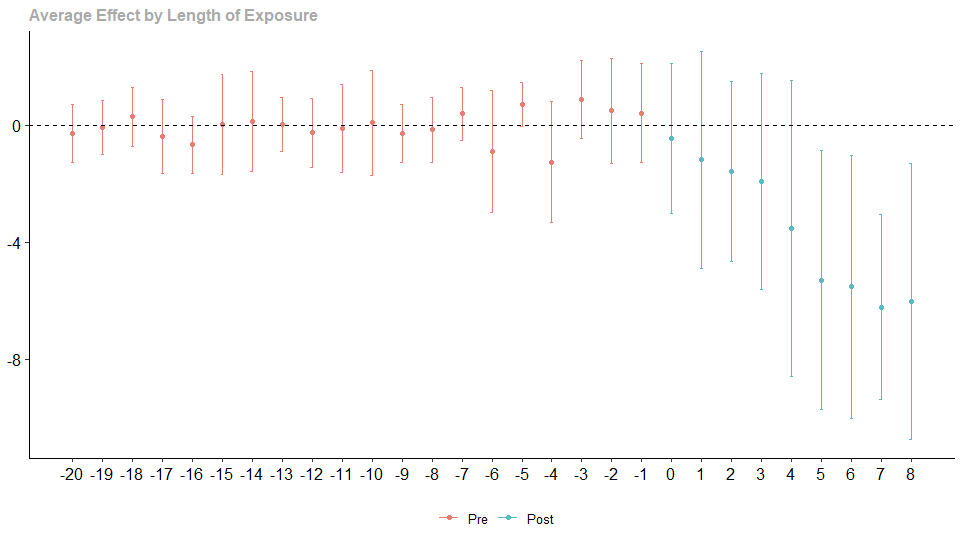
\includegraphics[width=.85\textwidth]{sc_graph.png}
    \end{center}
    \caption{ATT of treatment year on opioid death rate per 100k}
    \label{fig:graph}
\end{figure}


%------------------------------------------------------------------------------------------------

\section*{Discussion}

As expected, opioid deaths goes down. Marijuana becomes a substitute for opioids. 

More liberal states may be more likely to legalize Marijuana.

%------------------------------------------------------------------------------------------------

\section*{Conclusion}

Marijuana legalization leads to less opioid deaths. Legalizing marijuana can save lives. 


%----------------------------------------------------------------------------------------

\end{document}
